\section{数据理解与总体思路}

\subsection{数据来源与结构}

附件提供了某地区（多为高 BMI）孕妇的 NIPT 数据，含两个工作表：

\begin{itemize}
  \item \textbf{男胎检测数据}：1082 条检测记录、31 个字段，来自 267 名孕妇（每名孕妇多次采血检测，为纵向面板数据）。
  \item \textbf{女胎检测数据}：605 条检测记录、31 个字段，来自 147 名孕妇。
\end{itemize}

关键字段包括：孕妇年龄、身高、体重、检测孕周（字符串形式，如 ``11w+6''）、孕妇 BMI、Y 染色体浓度、X 染色体浓度、13/18/21/X 染色体的 Z 值、13/18/21 染色体的 GC 含量、原始读段数、唯一比对读段数、重复读段比例、被过滤读段数比例、染色体非整倍体（空白即无异常）、胎儿是否健康等。

\subsection{数据预处理}

\begin{enumerate}
  \item \textbf{孕周解析}：将 ``11w+6''、``16W+1'' 等字符串统一解析为连续数值周（周 + 天/7），无解析失败。
  \item \textbf{缺失处理}：男胎 ``染色体的非整倍体'' 缺失表示无异常（正常标签）；女胎 Y 染色体浓度与 Y 染色体 Z 值两列全空，符合女胎无 Y 染色体的生理事实。
  \item \textbf{派生指标}：构造 ``达标''（Y 浓度是否 $\ge 4\%$）、``个体达标时间''（Y 浓度首次达到 4\% 的孕周）等指标。
\end{enumerate}

数据处理与特征构造流程如图~\ref{fig:pipeline} 所示。

\begin{figure}[H]
  \centering
  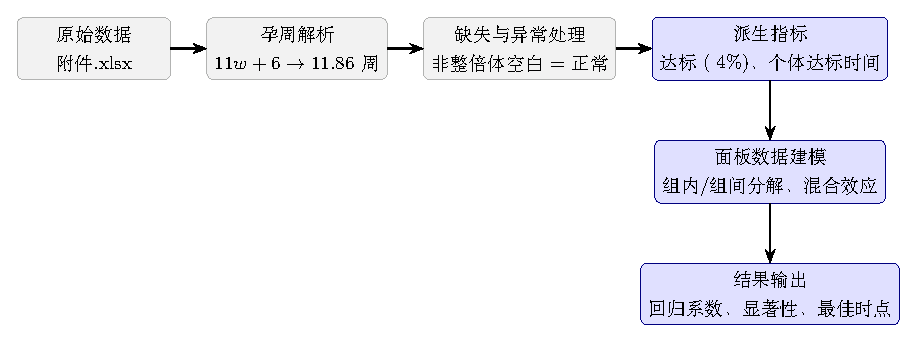
\includegraphics[width=0.85\textwidth]{../figures/fig_pipeline.pdf}
  \caption{数据清洗与特征构造流程}
  \label{fig:pipeline}
\end{figure}

\subsection{总体建模思路}

本题为统计建模与分类判定相结合的题型，整体技术路线如图~\ref{fig:roadmap} 所示。核心思路是：先通过面板数据（纵向重复测量）方法分离孕周与 BMI 对 Y 染色体浓度的影响（问题一）；在此基础上估计每位孕妇的达标时间，据以对 BMI（问题二）或多维因素（问题三）分组并给出风险最小的最佳 NIPT 时点；最后针对女胎建立异常判定的分类模型（问题四）。

\begin{figure}[H]
  \centering
  
\includegraphics[width=0.9\textwidth]{../figures/fig_roadmap.pdf}
  \caption{本文整体建模技术路线}
  \label{fig:roadmap}
\end{figure}
